
In order to distinguish a quenched zone from a non-quenched one, the superconducting cable is divided into two domains as presented in Fig. \ref{fig:ansys_material_assignment}. The non-quenched part is characterised by nearly zero-resistivity (not zero for the sake of numerical stability) whereas the quenched cable has nonlinear resistivity of a strand composite as described in (\ref{eqn:strand_resistivity})~\cite{simon_mcintosh_private_communication}. The nonlinear resistivity is reassigned as the quench propagates in the numerical model.

\begin{figure}[H]
\centering
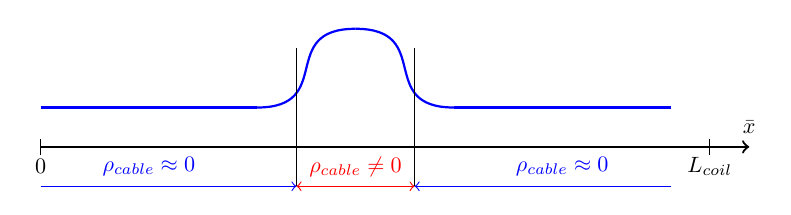
\begin{tikzpicture}[scale = 1]
\draw [thick, ->] (0.0,0.0) -- (9.0,0);
\draw [thick, blue] (0.0,0.5) -- (2.75,0.5);
\draw [thick, blue] (5.25,0.5) -- (8.0,0.5);
\draw [thick, blue] (2.75,0.5) .. controls +(0:1cm) and +(180:1cm) .. (4.0,1.5);
\draw [thick, blue] (4.0,1.5) .. controls +(0:1cm) and +(180:1cm) .. (5.25,0.5);

\draw [thin, red, <->] (3.25,-0.5) -- (4.75,-0.5);
\draw [thin, blue, ->] (0.0,-0.5) -- (3.25,-0.5);
\draw [thin, blue, <-] (4.75,-0.5) -- (8.0,-0.5);

\node[scale = 0.8] [color = red] at (4.0,-0.25) {$\rho_\text{cable} \neq 0$};
\node[scale = 0.8] [color = blue] at (1.375,-0.25) {$\rho_\text{cable} \approx 0$};
\node[scale = 0.8] [color = blue] at (6.625,-0.25) {$\rho_\text{cable} \approx 0$};

\node[scale = 0.8] at (9.0,+0.25) {$\bar x$};
\node[scale = 0.8] at (8.5,-0.25) {$L_\text{coil}$};
\draw [thin] (8.5,-0.10) -- (8.5,0.10);
\draw [thin] (0,-0.10) -- (0,0.10);
\node[scale = 0.8] at (0,-0.25) {0};

\draw [thin] (3.25,-0.5) -- (3.25,1.25);
\draw [thin] (4.75,-0.5) -- (4.75,1.25);

\end{tikzpicture}
\caption{Material properties assignment in ANSYS depending on the quenched and non-quenched zone~\cite{simon_mcintosh_private_communication}.}
    \label{fig:ansys_material_assignment}
\end{figure}

The reassignment of material properties is handled by an external routine which controls the quench propagation in time. In this case, a thermal model (solved by the numerical model) and quench velocity estimator (calculated by the external routine) are co-simulated. This problem can be resolved by means of: 

\begin{enumerate}
    \item one-directional exchange of signals;
    \item bi-directional exchange of signals.
\end{enumerate}

The one-directional exchange of signals is presented in Fig. \ref{fig:unidirectional_coupling_scheme}. In this case, the numerical solver is provided with a quench front position from the previous communication point $t_{j-1}$ and calculates the temperature distribution in the current communication point~$t_j$. The parameter denoted as $x_{j-1}$ represents the information about the value of the next communication point $t_j$ and the quench front position in the cable. The external routine assumes a constant quench velocity independent of current and magnetic field strength. Therefore, the routine is not updated.

\begin{figure}[H]
\centering
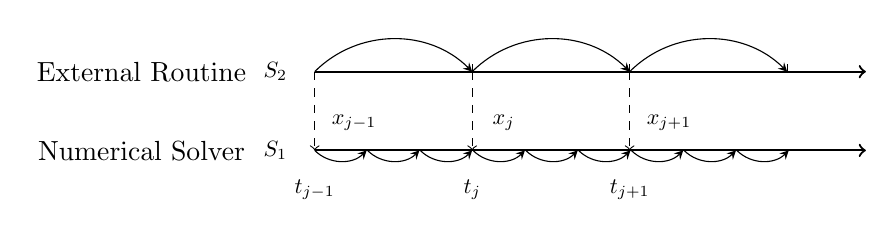
\begin{tikzpicture}[scale = 1]
\draw[thick,->] (0,1) -- (7,1);
\draw (2, 1) -- (2, 1.1);
\draw (4, 1) -- (4, 1.1);
\draw (6, 1) -- (6, 1.1);
\foreach \t in {1,3,5}
\draw [-stealth, bend angle=45, bend left, color = black]  ({\t-1},1) to (\t+1,1);
\draw[thick,->] (0,0) -- (7,0);
\draw (2, 1) -- (2, 1.1);
\draw (4, 1) -- (4, 1.1);
\draw (6, 1) -- (6, 1.1);
\foreach \t in {0.66,1.33,...,6.33}
\draw [-stealth, bend angle=45, bend right]  ({\t-0.66},0) to (\t,0);
\node[scale = 0.8] at (0, -0.5) {$t_{j-1}$};
\node[scale = 0.8] at (2,-0.5) {$t_j$};
\node[scale = 0.8] at (4,-0.5) {$t_{j+1}$};
\draw[dashed, ->] (0,1) -- (0,0);
\draw[dashed, ->] (2,1) -- (2,0);
\draw[dashed, ->] (4,1) -- (4,0);
\node[scale = 0.8] at (-0.5, 0) {$\text{S}_1$};
\node[scale = 0.8] at (-0.5, 1) {$\text{S}_2$};
\node[scale = 0.8] at (0.5, 0.35) {$x_{j-1}$};
\node[scale = 0.8] at (2.4, 0.35) {$x_{j}$};
\node[scale = 0.8] at (4.5, 0.35) {$x_{j+1}$};
\node[color = black] at (-2.2,1.0)	{External Routine};
\node at (-2.2,0)	{Numerical Solver};
\end{tikzpicture}
\caption{Schematic representation of one-directional coupling between a numerical solver and the quench velocity estimator.}
\label{fig:unidirectional_coupling_scheme}
\end{figure}

The bi-directional exchange of signals is presented in Fig. \ref{fig:bidirectional_coupling_scheme}.
Additionally to the one-directional case, the external routine is updated with the value of current and magnetic field strength from the numerical solver denoted as $y_j$ at communication point $t_j$ to estimate the quench velocity at $t_{j-1}$.

\begin{figure}[H]
\centering
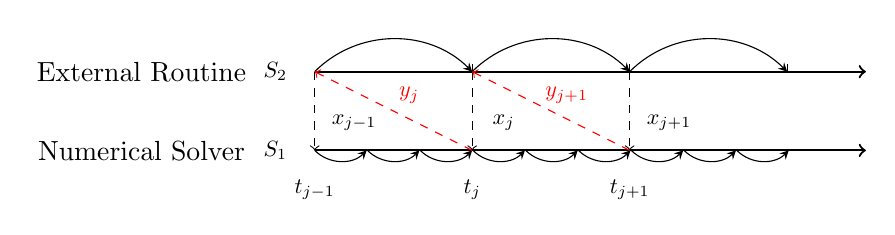
\begin{tikzpicture}[scale = 1]
\draw[thick,->] (0,1) -- (7,1);
\draw (2, 1) -- (2, 1.1);
\draw (4, 1) -- (4, 1.1);
\draw (6, 1) -- (6, 1.1);
\foreach \t in {1,3,5}
\draw [-stealth, bend angle=45, bend left, color = black]  ({\t-1},1) to (\t+1,1);
\draw[thick,->] (0,0) -- (7,0);
\draw (2, 1) -- (2, 1.1);
\draw (4, 1) -- (4, 1.1);
\draw (6, 1) -- (6, 1.1);
\foreach \t in {0.66,1.33,...,6.33}
\draw [-stealth, bend angle=45, bend right]  ({\t-0.66},0) to (\t,0);
\node[scale = 0.8] at (0, -0.5) {$t_{j-1}$};
\node[scale = 0.8] at (2,-0.5) {$t_j$};
\node[scale = 0.8] at (4,-0.5) {$t_{j+1}$};
\draw[dashed, ->] (0,1) -- (0,0);
\draw[dashed, ->] (2,1) -- (2,0);
\draw[dashed, ->] (4,1) -- (4,0);
\draw[dashed, red, ->] (2,0) -- (0,1);
\draw[dashed, red, ->] (4,0) -- (2,1);
\node[scale = 0.8] at (-0.5, 0) {$\text{S}_1$};
\node[scale = 0.8] at (-0.5, 1) {$\text{S}_2$};
\node[scale = 0.8] at (0.5, 0.35) {$x_{j-1}$};
\node[scale = 0.8] at (2.4, 0.35) {$x_{j}$};
\node[scale = 0.8] at (4.5, 0.35) {$x_{j+1}$};
\node[scale = 0.8, red] at (1.2, 0.7) {$y_{j}$};
\node[scale = 0.8, red] at (3.2, 0.7) {$y_{j+1}$};
\node[color = black] at (-2.2,1.0)	{External Routine};
\node at (-2.2,0)	{Numerical Solver};
\end{tikzpicture}
\caption{Schematic representation of bi-directional coupling between a numerical solver and the quench velocity estimator.}
\label{fig:bidirectional_coupling_scheme}
\end{figure}

In both cases, the initial quench length is assumed at the beginning of the co-simulation. Between the time steps of the external routine, the numerical solver handles the problem with an adaptive time step smaller than the communication points $t_j$.

Provided that the data exchange between an external routine and a numerical solver occurs at communication times $t_j$, the quench velocity assignment algorithm is solved as described in Algorithm~\ref{alg:weak_coupling}.

\begin{algorithm}[H]
  \caption{Quench velocity assignment algorithm.}
  \label{alg:weak_coupling}
  \begin{algorithmic}[1]
    \STATE assume initial quench position $x_{j-1}$ 
    \STATE \textbf{for} $j=1,2,...,N$ \textbf{do}
    \STATE \hspace{0.5cm} solve temperature distribution at time $t_j$
    \STATE \hspace{0.5cm} send solver results $y_{j}$ to external routine time $t_{j-1}$ (only for a bi-directional case)
    \STATE \hspace{0.5cm} calculate new quench position $x_{j}$ for a quench front
    \STATE \hspace{0.5cm} assign quench position $x_{j}$ to new nodes for solver time  $t_j$
  \end{algorithmic}
\end{algorithm}

To sum up, the quench velocity assignment algorithm only requires a one-directional exchange of signals at fixed current and magnetic field strength. If the quench simulation is conducted at varying values of current and/or magnetic field, the bi-directional exchange of signals must be implemented. In this thesis, the quench velocity is estimated numerically. In the following chapters, the communication times $t_j$ between ANSYS and the external routine are described as $t_\text{com}$.
